\documentclass{article}
\usepackage{graphicx,psfrag,epsfig,epsf,latexsym,hhline,amsmath,amssymb,multirow}
\usepackage[usenames,dvipsnames]{pstricks}
\usepackage{pst-plot}
\usepackage{pstricks-add}
\usepackage{color}
\usepackage{stmaryrd}
\usepackage{makecell}

\interdisplaylinepenalty=2500
\usepackage{graphicx}
\usepackage{amsthm}
\usepackage{footnote}
\usepackage{blindtext}
\usepackage{etoolbox}

\usepackage{tikz}
\usepackage{pgfplots}
\usepgflibrary{shapes}
\usetikzlibrary{matrix,positioning}
\usetikzlibrary{decorations.pathreplacing}
\usetikzlibrary{arrows,shapes,chains,matrix,positioning,scopes,patterns	}
\pgfplotsset{compat=newest}
\pgfplotsset{plot coordinates/math parser=false}

\begin{document}

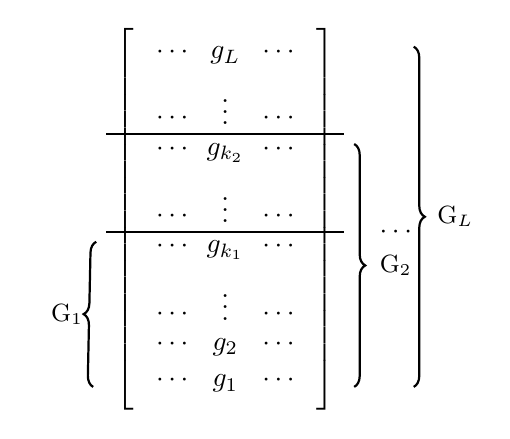
\begin{tikzpicture}

\matrix(mymatrix)[matrix of math nodes, left delimiter={[},right delimiter={]}]
	{
              \cdots & g_{L} & \cdots \\
              \cdots & \vdots & \cdots \\
%						\hline
              \cdots & g_{k_2} & \cdots \\
              \cdots & \vdots & \cdots \\
%						\hline
              \cdots & g_{k_1} & \cdots \\
              \cdots & \vdots & \cdots \\
              \cdots & g_2 & \cdots \\
              \cdots & g_1 & \cdots \\
	};        
\coordinate (la) at (mymatrix-1-1.north west);	
\coordinate (ra) at (mymatrix-1-3.north east);	

\coordinate (lb) at (mymatrix-2-1.south west);	
\coordinate (rb) at (mymatrix-2-3.south east);	

\coordinate (lc) at (mymatrix-4-1.south west);	
\coordinate (rc) at (mymatrix-4-3.south east);	

\coordinate (ld) at (mymatrix-8-1.south west);	
\coordinate (rd) at (mymatrix-8-3.south east);	
\def \offs{0.2in};

  \node (la_left)  [left = \offs of la]    {};    %Left coordinate outside the matrix for the 1st extended hline
  \node (ra_right)  [right = \offs of ra]    {};    %Right coordinate outside the matrix for the 1st extended hline
  \node (lb_left)  [left = \offs of lb]    {};    %Left coordinate outside the matrix for the 1st extended hline
  \node (rb_right)  [right = \offs of rb]    {};    %Right coordinate outside the matrix for the 1st extended hline
  \node (lc_left)  [left = \offs of lc]    {};    %Left coordinate outside the matrix for the 1st extended hline
  \node (rc_right)  [right = \offs of rc]    {};    %Right coordinate outside the matrix for the 1st extended hline
  \node (ld_left)  [left = \offs of ld]    {};    %Left coordinate outside the matrix for the 1st extended hline
  \node (rd_right)  [right = \offs of rd]    {};    %Right coordinate outside the matrix for the 1st extended hline

  \node (la_left_left)  [left = \offs of la_left]    {};    %Left coordinate outside the matrix for the 1st extended hline
  \node (ra_right_right)  [right = \offs of ra_right]    {};    %Right coordinate outside the matrix for the 1st extended hline
   \node (rd_right_right)  [right = \offs of rd_right]    {};    %Right coordinate outside the matrix for the 1st extended hline

%The two hlines in the Matrix
\draw[black,thick] (lb_left) -- (rb_right);
\draw[black,thick] (lc_left) -- (rc_right);


\draw [decorate,thick,decoration={brace,amplitude=4pt,mirror},xshift=5pt,yshift=0pt]
([xshift=-20pt]lc_left) -- ([xshift=-20pt]ld_left) node [black,midway,xshift=-10pt]{\small $\text{G}_{1}$};

\draw [decorate,thick,decoration={brace,amplitude=4pt},xshift=-10pt,yshift=0pt](rb_right) -- (rd_right) node [black,midway,xshift=15pt]{\small $\text{G}_{2}$};

\node [right= 0.5ex of rc_right] {$\cdots$};

\draw [decorate,thick,decoration={brace,amplitude=4pt},xshift=-10pt,yshift=0pt](ra_right_right) -- (rd_right_right) node [black,midway,xshift=15pt]{\small $\text{G}_{L}$};

%\draw [decorate,thick,decoration={brace,amplitude=4pt,mirror},xshift=-0.5in,yshift=0pt]
%(lb_left) -- (ld_left) node [black,midway,xshift=-19pt]{\small $\text{G}_{2}$};

        \end{tikzpicture}
\end{document}